\documentclass[a4paper, 12pt]{article}

\usepackage[UTF8]{ctex}
\usepackage{graphicx}
\usepackage{lipsum}
\usepackage[colorlinks=true]{hyperref}
\usepackage[margin=.5in]{geometry}

\begin{document}
\pagenumbering{gobble}

\large
\title{Java}
\author{Joshua Yu}
\date{11 July. 2019}
\maketitle
\tableofcontents

%\lipsum[1-5]

\section{Caveats}
\begin{itemize}
\item ``Intellij IDEA run button grayed out''?
\begin{enumerate}
\item Right click the folder containing your source
\item Select Mark Directory as $\rightarrow$ Test Source Root
\end{enumerate}

\item pre or post decrement won't work in a regular for loop at the iteration expression part
\begin{verbatim}
for (int y = 4; y > 2; y--) {
  System.out.println(y);
}
\end{verbatim}
and
\begin{verbatim}
for (int y = 4; y > 2; --y) {
  System.out.println(y);
}
\end{verbatim}
produce the same result

\end{itemize}


\section{FAQ}
\begin{enumerate}
\item 在constructor里面使用this和不使用this都一样吗?(在普通函数里面使用 instance fields 的时候不用this)

\item ArrayList的type如果是Integer,那么remove的时候写数字是移除对应的值还是对应index上的值?

移除其对应index上的值。因为写数字则其type为int类型,而非Integer类型,如果要移除对应的值则需要 \verb|cast| 为Integer类型。{\color{red}类型不同为什么用 \verb|cast| operator成功了呢?}

\item 在main方法里面可以直接使用 non-static instance variables 吗?

不行。因为main方法是 static method,不能直接使用 non-static instance variables

\item 下面程序在cmd里面打印的时候出现乱码
\begin{verbatim}
import java.util.Date;

public class TestFormats {
  public static void main (String [] args) {		
	  Date today = new Date();
	  System.out.printf(String.format("%tA, %tB %td", today, today, 
    today));
  }
}
\end{verbatim}

\end{enumerate}


\section{Hello World}
\subsection{Hello Java File!}
HelloYou.java

\begin{verbatim}
public class HelloYou {
  public static void main(String[] args) {
    System.out.println("Hello Joshua!");
  }
}
\end{verbatim}
\verb|println| is short for ``print line''. It has to be double quotes inside \verb|println|

\subsection{Commenting Code}
When comments are short we use the single-line syntax: \verb|//|.

When comments are long we use the multi-line syntax: \verb|/*| and \verb|*/|.

\subsection{Semicolons and Whitespace}
Java does not interpret \textit{whitespace}, the areas of the code without syntax, but humans use whitespace to read code without difficulty.

Java \textbf{does} interpret semicolons. Semicolons are used to mark the end of a statement, one line of code that performs a single task.

Let's contrast statements with the curly brace, \verb|{}|. Curly braces mark the scope of our classes and methods. There are no semicolons at the end of a curly brace.

\subsection{Compilation: Catching Errors}
with a file called Plankton.java, we could compile it with the terminal command:

\verb|javac Plankton.java|

A successful compilation produces a \verb|.class| file: \verb|Plankton.class|, that we execute with the terminal command:

\verb|java Plankton|


\section{Java Program Structure}
Java is a case-sensitive language.

\subsection{Classes}
All Java programs are made of at least one class. The class name must match the file: our file is \textbf{HelloWorld.java} and our class is \verb|HelloWorld|. We capitalize every word, a style known as \textit{pascal case}. Java variables and methods are named in a similar style called \textit{camel case} where every word \textbf{after the first} is capitalized.

\subsection{Methods}
Every Java program must have a method called \verb|main()|. A method is a sequence of tasks for the computer to execute. This \verb|main()| method holds all of the instructions for our program.

\href{https://github.com/twitter/commons/blob/master/src/java/com/twitter/common/styleguide.md#dont-embed-metadata-in-variable-names}{Don't embed metadata in variable names} seems differenct from JavaScript


\section{Variables}
\textit{Primitive datatypes} are types of data built-in to the Java system

\verb|int double boolean char|

The \verb|char| data type which store \textit{single character} can hold any character, like a letter, space, or punctuation mark. It must be surrounded by single quotes, '. For example:
\verb|char punctuation = '!';|

So far, we have learned primitive data types, which are the simplest types of data with no built-in behavior. Our programs will also use \verb|String|s, which store multiple characters using double quotes, which are objects, instead of primitives. Objects have built-in behavior.

A variable starts with a valid letter, or a \verb|$|, or a \verb|_|.


\section{Manipulating Variables}
With objects, such as \verb|String|s, we can't use the primitive equality operator. To test equality with \verb|String|s, we use a built-in method called \verb|.equals()|.
\subsection{String Concatenation}
The \verb|+| operator can be used to concatenate \verb|String|s.
\begin{verbatim}
// can be primitive datatype as well, Java will intelligently make it a 
// String first
String username = "PrinceNelson";
System.out.println("Your username is: " + username);
\end{verbatim}


\section{Introduction to Classes}
\subsection{Classes: Syntax}
The fundamental concept of object-oriented programming is the class. Every program has at least one class
\begin{verbatim}
public class Car {
// scope of Car class starts after curly brace

  public static void main(String[] args) {
    // scope of main() starts after curly brace

    // program tasks

  }
  // scope of main() ends after curly brace

}
// scope of Car class ends after curly brace
\end{verbatim}
This example defines a \verb|class| named \verb|Car|. \verb|public| is an \textit{access level modifier} that allows \textbf{other} classes to interact with this class.

\subsection{Classes: Constructors}
We create objects (instances of a class) using a constructor method. See java.pdf for an example

\subsection{Classes: Instance Fields}
We'll add associated data to an object by introducing instance variables, or instance fields. Instance fields are the state in our objects. See java.pdf for an example

Instance Fields are also available inside all methods {\color{red}(in main method, accessed by instance of the class)} in the class, since it is in the scope of the whole class.

\subsection{Classes: Constructor Parameters}
Parameters specify the type and name of data available for reference within a method's scope. See java.pdf for an example

\subsection{Classes: Assigning Values to Instance Fields}
Now that our constructor has a parameter, we must pass values into the method call. These values become the state of the instance. See java.pdf for an example


\section{Methods}
\subsection{Defining Methods}
\begin{verbatim}
public void startEngine() {
  System.out.println("Starting the car!");
  System.out.println("Vroom!");
}
\end{verbatim}
The first line, \verb|public void startEngine()|, is the method signature. It gives the program some information about the method:
\begin{itemize}
\item \verb|public| means that other classes can access this method

\item The \verb|void| keyword means that there is no specific output from the method (no value is returned)

\item \verb|startEngine()| is the name of the method

\end{itemize}

\subsection{Calling Methods}
When we add the \verb|startEngine()| method to the \verb|Car| class, it becomes available to use on any \verb|Car| object

\subsection{Reassigning Instance Fields}
In this codecademy example, \verb|price| is an instance field of type \verb|double|
\begin{verbatim}
// increase price method
public void increasePrice(double priceToAdd){
  double newPrice = price + priceToAdd;
  price = newPrice;
}
\end{verbatim}
why not just \verb|price = price + priceToAdd;|? 改成这个编译也可以

\subsection{Returns}
We can use a value outside of the method it was created in if we \textit{return} it from the method.
\begin{verbatim}
public int numberOfTires() {
   int tires = 4;
   return tires;
}
\end{verbatim}
In past exercises, when creating new methods, we used the keyword \verb|void|. Here, we are replacing \verb|void| with \verb|int|, to signify that the \textit{return type} is an \verb|int|.

\subsection{The toString() Method}
When we print out Objects, we often see a String that is not very helpful in determining what the Object represents: \verb|Store@6bc7c054|.

See java.pdf for an example


\section{Introduction to Control Flow}
\textit{if-then-else} statement:
\begin{itemize}
\item If \textit{condition} is true, then do something

\item Else, do a different thing

\end{itemize}

Only one of the code blocks will run.

\vspace{1.3em}

Switch Statement:

See java.pdf for an example. Switch blocks are different than other code blocks because they are not marked by curly braces and we use the \verb|break| keyword to exit the switch statement.

\subsection{Conditional Operators}
Conditional-AND, \verb|&&|, evaluates to \verb|true| if the booleans on both sides are \verb|true|.

Conditional-OR, $\vert\vert$, evaluates to \verb|true| if one or both of the booleans on either side is \verb|true|.

Logical-NOT, \verb|!|, evaluates to the opposite boolean value to which it is applied.


\section{Arrays}
Array indexes start at 0!

An array holds a fixed number of values of one type. Arrays hold \verb|double|s, \verb|int|s, \verb|boolean|s, or any other primitives. Arrays can also contain \verb|String|s, or any other objects!

\subsection{Creating an Array Explicitly}
we can declare and initialize in the same line:\\
\verb|double[] prices = {13.15, 15.87, 14.22, 16.66};|

\subsection{Importing Arrays}
\begin{verbatim}
String[] topics = {"Opinion", "Tech", "Science", "Health"};
System.out.println(topics);
\end{verbatim}
will print out \verb|[Ljava.lang.String;@2aae9190|

If we want to have a more descriptive printout of the array itself, we need a \verb|toString()| method that is provided by the \verb|Arrays| package in Java.\\
\verb|import java.util.Arrays;|

We put this at the top of the file, before we even define the class! Then once again if we print out \verb|Arrays.toString(topics)|, we'll get \verb|[Opinion, Tech, Science, Health]|

\subsection{Creating an Empty Array}
Empty arrays have to be initialized with a fixed size:\\
\verb|String[] menuItems = new String[5];|

Once you declare this size, it cannot be changed! This array will always be of size 5, the \verb|length| field (\verb|menuItems.length|) of the array object will be 5.


\section{ArrayLists}
When we work with arrays in Java, we've been limited by the fact that once an array is created, it has a fixed size. We can't add or remove elements.

To represent dynamic lists, we can use Java's ArrayLists. ArrayLists allow us to:
\begin{itemize}
\item Store elements of the same type (just like arrays)

\item Access elements by index (just like arrays)

\item Add elements

\item Remove elements

\end{itemize}

\verb|import java.util.ArrayList;|

\subsection{Creating ArrayLists}
\verb|ArrayList<String> babyNames;|

We use angle brackets \verb|<| and \verb|>| to declare the type of the \verb|ArrayList|. These symbols are used for \textit{generics}.

See page 287 of ``Head First Java 2.0".

Generics are a Java construct that allows us to define classes and objects as parameters of an \verb|ArrayList|. For this reason, we can't use primitive types in an \verb|ArrayList|:
\begin{verbatim}
// This code won't compile:
ArrayList<int> ages;

// This code will compile:
ArrayList<Integer> ages;
\end{verbatim}
The \verb|<Integer>| generic has to be used in an \verb|ArrayList| instead. You can also use \verb|<Double>| and \verb|<Char>| for types you would normally declare as \verb|double|s or \verb|char|s.

We can initialize to an empty \verb|ArrayList| using the \verb|new| keyword:
\begin{verbatim}
// Declaring:
ArrayList<Integer> ages;
// Initializing:
ages = new ArrayList<Integer>();

// Declaring and initializing in one line:
ArrayList<String> babyNames = new ArrayList<String>();
\end{verbatim}


\subsection{Adding an Item}
\verb|ArrayList| comes with an \verb|add()| method that takes an argument to add to the end of the \verb|ArrayList|:
\begin{verbatim}
ArrayList<String> toDoList = new ArrayList<String>();
String toDo1 = "Water plants";
// Add more to-dos here:
String toDo2 = "feed cat";
String toDo3 = "walk the dog";

// Add to-dos to toDoList
toDoList.add(toDo1);
toDoList.add(toDo2);
toDoList.add(toDo3);
\end{verbatim}

To get ArrayList size, we use \verb|size()| method.

\subsection{Accessing an Index}
For \verb|ArrayList|s, bracket notation won't work. Instead, we use the method \verb|get()| to access an index:
\begin{verbatim}
// Print out the toDoList's second item
System.out.println(toDoList.get(1));
\end{verbatim}

\subsection{Changing a Value and Removing an Item}
When we were using arrays, we could rewrite entries by using bracket notation to reassign values.

\verb|ArrayList| has a slightly different way of doing this, using the \verb|set()| method:
\begin{verbatim}
ArrayList<String> shoppingCart = new ArrayList<String>();

shoppingCart.add("Trench Coat");
shoppingCart.add("Tweed Houndstooth Hat");
shoppingCart.add("Magnifying Glass");

shoppingCart.set(0, "Tweed Cape");

// shoppingCart now holds ["Tweed Cape", "Tweed Houndstooth Hat", "Magnifying Glass"]
\end{verbatim}

To remove the first item of shoppingCart we write:\\
\verb|shoppingCart.remove(0);| or \verb|shoppingCart.remove("Trench Coat");| (this command removes the FIRST instance of the value ``Trench Coat'')

\subsection{Getting an Item's Index}
\begin{verbatim}
// detectives holds ["Holmes", "Poirot", "Marple", "Spade", "Fletcher", 
// "Conan", "Ramotswe"];
System.out.println(detectives.indexOf("Fletcher"));
\end{verbatim}
This code would print 4


\section{Loops}
\subsection{Iterating Over Arrays and ArrayLists}
Iterate over Arrays
\begin{verbatim}
for (int i = 0; i < secretCode.length; i++) {
  secretCode[i] += 1;
}
\end{verbatim}

Iterate over ArrayLists
\begin{verbatim}
for (int i = 0; i < secretCode.size(); i++) {
  int num = secretCode.get(i);
  secretCode.set(i, num + 1);
}
\end{verbatim}

\subsection{For-Each Loops}
For-each loops allow you to directly loop through each item in a list of items (like an array or ArrayList) and perform some action with each item. The syntax looks like this:
\begin{verbatim}
for (String inventoryItem : inventoryItems) {
  System.out.println(inventoryItem);
}
\end{verbatim}
We can read the \verb|:| as ``in'' like this: for each \verb|inventoryItem| (which should be a \verb|String|) in \verb|inventoryItems|, print \verb|inventoryItem|


\section{String Methods}
In this lesson, we will go over several string methods:\\
\verb|length()  concat()  equals()  indexOf()  charAt()  substring()|\\
\verb|toUpperCase() / toLowerCase()|

In theory, the \verb|length| of a String is the same as the Unicode units of the String. For example, escape sequences such as \verb|\n| count as only one character.

\verb|concat()| doesn't actually change the value of the original string.

If the \verb|indexOf()| doesn't find what it's looking for (could be a letter or an entire substring), it'll return a $-1$.

The \verb|charAt()| method returns the character located at a \verb|String|'s specified index, if the index is out of str's range, it will produce an error.

\verb|substring()| returns a string that is a substring of this string. There're two variants:
\begin{itemize}
\item \verb|substring(int beginIndex)|, eg. \verb|"unhappy".substring(2) returns "happy"|

\item \verb|substring(int beginIndex, int endIndex)|, the substring begins at the specified \verb|beginIndex| and extends to the character at index \verb|endIndex - 1|\\ eg. \verb|"smiles".substring(1, 5) returns "mile"|

\end{itemize}

\verb|toUpperCase() / toLowerCase()| return the string value converted to uppercase or lowercase. A good use of this functionality is to ensure consistency of the data you store in a database.


\section{Inheritance and Polymorphism}
There are several terms you'll encounter frequently:
\begin{itemize}
\item \textit{Parent class}, \textit{superclass}, and \textit{base class} refer to the class that another class inherits from (like Shape)

\item \textit{Child class}, \textit{subclass}, and \textit{derived class} refer to a class that inherits from another class (like Triangle)

\end{itemize}

\subsection{Inheritance in Practice}
We use the keyword \verb|extends| like this:
\begin{verbatim}
class Shape {

  // Shape class members

}

class Triangle extends Shape {

  // additional Triangle class members

}
\end{verbatim}

child class inherits its parent's fields and methods

\subsection{Inheriting the Constructor}
child class inherits its parent's constructor as well. 

Using the \verb|super()| method which acts like the parent constructor inside the child class constructor. See java.pdf for an example.

It is also possible to just completely override a parent class constructor by writing a new constructor for the child class:
\begin{verbatim}
class Triangle extends Shape {
  Triangle() {
    this.numSides = 3;
  }

  // additional Triangle class members

}
\end{verbatim}
Turns out I still have to add \verb|super()| with related params first, then override \verb|numSides| field by writing \verb|this.numSides = 3;| after \verb|super()|.

\subsection{Parent Class Aspect Modifiers}
A child class does not inherit its parent's \verb|private| members

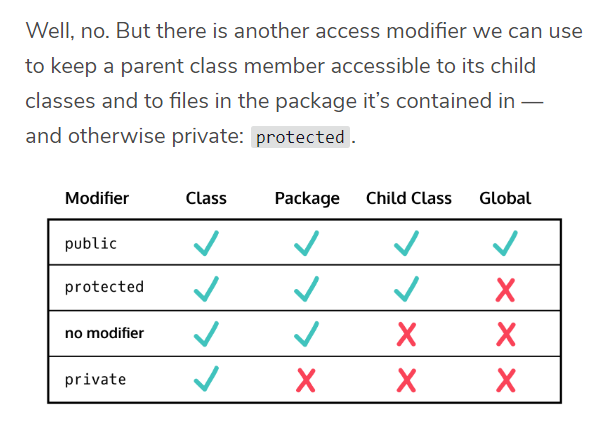
\includegraphics[width=12cm]{pics/accessModifiers.png}

package means files are under the same folder.

In addition to access modifiers, there's another way to establish how child classes can interact with inherited parent class members: using the \verb|final| keyword. If we add \verb|final| before a parent class method's access modifier, we disallow any child classes from changing that method. This is helpful in limiting bugs that might occur from modifying a particular method.

\textbf{Note:} If a class has no modifier (the default, also known as package-private), it is visible only within its own package.

The following figure shows the four classes in this example and how they are related.

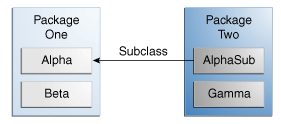
\includegraphics[width=8cm]{pics/classes-access.png}

The following table shows where the members of the Alpha class are visible for each of the access modifiers that can be applied to them.
\begin{table}[htbp]
\centering
\caption{Visibility}
\begin{tabular}{lllll}
Modifier & Alpha & Beta & AlphaSub & Gamma \\ \hline
public & Y & Y & Y & Y \\ \hline
protected & Y & Y & Y & N \\ \hline
no modifier & Y & Y & N & N \\ \hline
private & Y & N & N & N \\ \hline
\end{tabular}
\end{table}

\subsection{Method Overriding}
One common use of polymorphism with Java classes is something we mentioned earlier -- \textit{overriding} parent class methods in a child class.

Method Overriding: see java.pdf for an example. In order to properly override parent's methods {\color{red}(including constructor method using \verb|super()|)}, following has to be satisfied
\begin{itemize}
\item Method name

\item Return type

\item Number and type of parameters

\end{itemize}
does child's \verb|super()| has to satisfy the third item in order to properly override its parent's constructor method? Yes (concluded from the dinner project)

\subsection{Using a Child Class as its Parent Class}
An important facet of polymorphism is the ability to use a child class object where an object of its parent class is expected. See java.pdf for an example.

Method overriding is handled at runtime. If BiangBiang class have a method that Noodle class does	not have, then \verb|biangBiang| can not use that method, but can use any methods inside Noodle class.

\subsection{Child Classes in Arrays and ArrayLists}
Usually, when we create an array or an ArrayList, the list items all need to be the same type. But polymorphism puts a new spin on what is considered the same type...

In fact, we can put instances of different classes that share a parent class together in an array or \verb|ArrayList|! For example, let's say we have a \verb|Monster| parent class with a few child classes: \verb|Vampire|, \verb|Werewolf|, and \verb|Zombie|. We can set up an array with instances of each:
\begin{verbatim}
Monster dracula, wolfman, zombie1;

dracula = new Vampire();
wolfman = new Werewolf();
zombie1 = new Zombie();

Monster[] monsters = {dracula, wolfman, zombie1};
\end{verbatim}

We can even iterate through the list of items — regardless of subclass — and perform the same action with each item:
\begin{verbatim}
for (Monster monster : monsters) {
  monster.attack();
}
\end{verbatim}
In the code above, we were able to call \verb|attack()| on each monster in \verb|monsters| despite the fact that, in the for-each loop, monster is declared as the parent class type \verb|Monster|.

See java.pdf for an example.


\section{Debugging}
In Java, there are many different ways of classifying errors, but they can be boiled down to three categories:
\begin{itemize}
\item \textbf{Syntax errors}: Errors found by the compiler.

\item \textbf{Run-time errors}: Errors that occur when the program is running.

\item \textbf{Logic errors}: Errors found by the programmer looking for the causes of erroneous results.

\end{itemize}

\subsection{Run-time Errors}
If our program has no compile-time errors, it'll run. Errors which happen during program execution (run-time) after successful compilation are called run-time errors.

Some common run-time errors:
\begin{itemize}
\item Division by zero also known as division error

\item Trying to open a file that doesn't exist

\end{itemize}

\subsection{Exceptions}
\begin{itemize}
\item \verb|ArithmeticException|: Something went wrong during an arithmetic operation; for example, division by zero.

\item \verb|NullPointerException|: You tried to access an instance variable or invoke a method on an object that is currently \verb|null|.

\item \verb|ArrayIndexOutOfBoundsException|: The index you are using is either negative or greater than the last index of the array (i.e., \verb|array.length-1|).

\item \verb|FileNotFoundException|: Java didn't find the file it was looking for.

\end{itemize}

\subsection{Exception Handling}
One way to handle exceptions is using the \verb|try/catch|:
\begin{itemize}
\item The \verb|try| statement allows you to define a block of code to be tested for errors while it is being executed.

\item The \verb|catch| statement allows you to define a block of code to be executed if an error occurs in the try block.

\end{itemize}
\begin{verbatim}
public class Debug {
  public static void main(String[] args) {    
    int width = 0;
    int length = 40;
    
    try {
      int ratio = length / width;
    } catch (ArithmeticException e) {
      System.err.println(e.getMessage());
    }    
  }  
}
\end{verbatim}
An exception handler is considered appropriate if the type of the exception object thrown matches the type that can be handled by the handler.

You can also chain exceptions together:
\begin{verbatim}
try {
  //  Block of code to try
} catch (NullPointerException e) {
  //  Code to handle a NullPointerException
} catch (ArithmeticException e) {
  //  Code to handle an ArithmeticException
}
\end{verbatim}


\section{sql from Codecademy}
\subsection{Setting Up SQLite}
Binaries for SQLite can be installed at the \href{https://www.sqlite.org/download.html}{SQLite Download} page.

For Windows machines:
\begin{enumerate}
\item Download the \verb|sqlite-tools-win32-x86-3200100.zip| file and unzip it.

\item From your git-bash terminal, open the directory of the unzipped folder with \verb|cd ~/Downloads/sqlite-tools-win32-x86-3200100/|.

\item Try running sqlite with the command \verb|winpty ./sqlite3.exe|. If that command opens a \verb|sqlite>| prompt, congratulations! You've installed SQLite.

\end{enumerate}
We want to be able to access this command quickly from elsewhere, so we're going to create an alias to the command. Exit the \verb|sqlite>| prompt by typing in \verb|Ctrl + C|, and in the same git-bash terminal without changing folders, run these commands:\\
\verb|echo "alias sqlite3=\"winpty ${PWD}/sqlite3.exe\"" >> ~/.bashrc|\\
and\\
\verb|source ~/.bashrc|\\
The first command will create the alias \verb|sqlite3| that you can use to open a database. The second command will refresh your terminal so that you can start using this command. Try typing in the command \verb|sqlite3 newdb.sqlite|. If you're presented with a \verb|sqlite>| prompt, you've successfully created the \verb|sqlite3| command for your terminal. Enter \verb|Ctrl + C| to quit. You can also exit by typing \verb|.exit| in the prompt and pressing \verb|Enter|.

\subsection{How is ALTER different from UPDATE?}
Although similar in the sense that both statements will modify a table, these statements are quite different.

The \verb|ALTER| statement is used to modify columns. With \verb|ALTER|, you can add columns, remove them, or even modify them.

The \verb|UPDATE| statement is used to modify rows. However, \verb|UPDATE| can only update a row, and cannot remove or add rows.



\section{sql from w3schools}
\subsection{Combining AND, OR and NOT}
The following SQL statement selects all fields from ``Customers" where country is NOT ``Germany" and NOT ``USA":
\begin{verbatim}
SELECT * FROM Customers
WHERE NOT Country='Germany' AND NOT Country='USA';
\end{verbatim}

下面的sql语句不行
\begin{verbatim}
SELECT * FROM Customers 
WHERE NOT (Country='Germany' AND Country='USA');
\end{verbatim}

see java.pdf for a colorful code example.

\subsection{BETWEEN with IN Example}
See java.pdf for an example.

\subsection{RIGHT JOIN}
See java.pdf for an example.

\subsection{SELECT INTO}
\verb|SELECT INTO| can also be used to create a new, empty table using the schema of another. Just add a WHERE clause that causes the query to return no data:
\begin{verbatim}
SELECT * INTO newtable
FROM oldtable
WHERE 1 = 0;
\end{verbatim}



\href{http://www.nthuleen.com/teach/misc/typingumlauts.html}{Typing Umlauts on a PC and Mac}


\section{Miscellaneous}

\begin{enumerate}
\item 从JDK5.0开始,不再叫J2SE, 改名为Java SE了,因为那个2已经失去了其应该有的意义

\item MySql用得比较多

\item 在谈到Java开发人员经常使用的Java版本时,Java 8是胜利者。但应该记住,在2019年1月之后,Java 8(也就是jdk8) 将不再有公开更新。谈到Java开发人员最经常使用的IDE/编辑器时,IntelliJ IDEA看起来是明显的赢家。 \url{https://www.sohu.com/a/235541971_100159565}

\item winscp下载地址:\url{https://winscp.net/eng/download.php}

\item putty下载地址:\url{https://www.chiark.greenend.org.uk/~sgtatham/putty/latest.html}

\end{enumerate}

\end{document}




